\documentclass[10pt,twocolumn]{article}
\usepackage[margin=0.68in,columnsep=0.24in]{geometry}
\usepackage[T1]{fontenc}
\usepackage[utf8]{inputenc}
\usepackage{lmodern}
\usepackage{microtype}
\usepackage{amsmath,amssymb,amsthm}
\usepackage{booktabs}
\usepackage{graphicx}
\usepackage{xcolor}
\usepackage{enumitem}
\usepackage{hyperref}

\hypersetup{
  colorlinks=true,
  linkcolor=blue!60!black,
  citecolor=blue!60!black,
  urlcolor=blue!60!black,
  pdftitle={Certified Verification of Envy-Free Cake-Cutting for Five Agents},
  pdfauthor={Lluis Eriksson}
}

\newtheorem{proposition}{Proposition}
\newcommand{\QQ}{\mathbb{Q}}
\newcommand{\ZZ}{\mathbb{Z}}
\newcommand{\NN}{\mathbb{N}}
\newcommand{\ellv}{\boldsymbol{\ell}}

\title{\vspace{-1.1em}\textbf{Certified Verification of Envy-Free Cake-Cutting for Five Agents}}
\author{Lluis Eriksson\thanks{Independent Researcher. Code, Lean~4 proofs, and certificates: MIT License; manuscript and figures: CC-BY-4.0. Prepared with AI coding, formalization, and drafting assistance from Google Antigravity; all proofs, exact-$\QQ$ verifiers, and adversarial tests were independently compiled and verified locally. Repository: \url{https://github.com/lluiseriksson/envy-free-cake5-certificates}}}
\date{November 25, 2026}

\begin{document}
\maketitle
\vspace{-1.4em}

\begin{abstract}
Aris Filos-Ratsikas, Alexandros Hollender, Mohamad Latifian, and Giannis Tyrovolas (\texttt{arXiv:2611.33149}, Nov.\ 2026) resolved the open polylogarithmic query-complexity problem for five-agent contiguous $\varepsilon$-envy-free cake cutting under monotone Lipschitz valuations, achieving $O(\log^3(1/\varepsilon))$ value queries and a purely intermediate-value-theorem existence proof---via an algorithm obtained through interactions with ChatGPT~6~Astra. Their construction parameterizes four retained pieces $P_1, P_2, P_3, P_4$ plus two potential gaps $L, R$ around an anchor cut $m \in [0, 1]$ subject to maximal feasibility ($\ell_1 + \ell_2 = m$ or $\ell_3 + \ell_4 = 1 - m$), leaving-agent Hall robustness, softmax weight balancing ($W_j = 5/4$, non-favourite cap $2^{-5} = 1/32$), quantitative stability ($3\gamma^{-3}\delta$) and Lipschitz continuity ($13\gamma^{-3}$), and spanning-tree bisection ($O(\log^3(1/\varepsilon))$ vs.\ $O(\log^5(1/\varepsilon))$). We present a standalone, zero-dependency \textbf{Lean~4.35.0} formalization of 18 core combinatorial, Hall-margin, stability, Lipschitz, and bisection theorems (zero \texttt{sorry}, zero warnings, zero \texttt{Classical.choice}) paired with an exact-$\QQ$ four-mode certificate verifier (\texttt{EF-CAKE5-CERT-1.0}). Across 16 canonical certificates ($0.246$--$0.934\,\mathrm{ms}$, total $7.80\,\mathrm{ms}$), all invariants replay identically over $\QQ$ while rejecting 60/60 live adversarial forgery attacks.
\end{abstract}

\section{Introduction}\label{sec:intro}
Contiguous envy-free cake cutting guarantees that every agent receives a single interval of $[0, 1]$ and weakly prefers her own piece to any other~\cite{stromquist1980cut,su1999rental}. For monotone Lipschitz interval valuations, prior polylogarithmic-query algorithms reached three agents in $O(\log^2(1/\varepsilon))$ queries~\cite{deng2012algorithmic} and four agents in $O(\log^3(1/\varepsilon))$ queries~\cite{hollender2025envyfree4}, leaving five agents open. Filos-Ratsikas et al.~\cite{filosratsikas2026envyfree5} resolved the five-agent case in $O(\log^3(1/\varepsilon))$ value queries (Theorem~2) and gave a Sperner-free existence proof (Theorem~1) built on four interlocking pillars:
\begin{enumerate}[leftmargin=*,nosep]
  \item \textbf{Anchor Cut \& Maximal Leaving-Agent Robustness (Defs.~3.1--3.3, Lemmas~3.4--3.5):} For anchor $m \in [0,1]$, retained pieces $P_1 = [0,\ell_1], P_2 = [m-\ell_2, m], P_3 = [m, m+\ell_3], P_4 = [1-\ell_4, 1]$ leave gaps $L = [\ell_1, m-\ell_2]$ and $R = [m+\ell_3, 1-\ell_4]$; maximality enforces $L = \emptyset$ or $R = \emptyset$. Leaving-agent $\delta$-robustness~\cite{meunier2019multilabeled} holds iff Hall's condition holds after removing any agent $i \in [5]$ in $G_\delta(m, \ellv)$, forcing $G_\delta(m, \ellv)$ to be connected.
  \item \textbf{Softmax Weight Balancing (Lemmas~3.7 \& 3.9):} With $w_{ij} \propto 2^{(5/\delta)v_i(P_j)}$ ($\sum_{j=1}^4 W_j = 5$), balancing $W_j = 5/4$ bounds non-$\delta$-favourite weights by $2^{-5} = 1/32$, yielding $\lceil \frac{5}{4}|P| - 1 - 4|P|2^{-5}\rceil = \lceil (9|P|-8)/8\rceil \ge |P|$ for all $|P| \in \{1,2,3,4\}$.
  \item \textbf{Stability \& Lipschitz Continuity (Lemmas~3.17 \& 3.18):} Under $\gamma$-strong hungriness, any maximal $\delta$-robust tuple satisfies $\|\ellv - \ellv^*(m)\|_\infty \le 3\gamma^{-3}\delta$ and $m \mapsto \ellv^*(m)$ is $(13\gamma^{-3})$-Lipschitz.
  \item \textbf{Spanning-Tree Bisection (Lemmas~4.2--4.4, Thm.~2):} Enumerating the constant family of 8-edge spanning trees $T \subseteq G_0(\ellv^*(m))$ reduces five nested binary searches ($O(\log^5(1/\varepsilon))$) to $O(\log^3(1/\varepsilon))$ queries, with outer bisection tolerance $\varepsilon\gamma^3/156$ and strong-hungriness transfer $\gamma = \delta = \varepsilon/3 \implies \delta + 2\gamma = \varepsilon$.
\end{enumerate}

\paragraph{Contributions and Scope.}
We do not re-formalize continuous intermediate-value-theorem or compactness arguments inside Lean~4; instead, we machine-check every discrete, rational, graph-theoretic, and quantitative constant of~\cite{filosratsikas2026envyfree5}:
(i)~18 zero-\texttt{sorry}, zero-\texttt{Classical.choice} \textbf{Lean~4.35.0}~\cite{demoura2021lean4} theorems in \texttt{EnvyFreeCake5.lean};
(ii)~the exact-$\QQ$ four-mode certificate verifier \texttt{EF-CAKE5-CERT-1.0};
(iii)~16 canonical sub-millisecond certificates spanning all four modes; and
(iv)~a 60-attack live adversarial red-team suite with 41-artifact SHA-256 manifest enforcement.

\section{Constructive Lean~4.35.0 Kernel}\label{sec:lean}
The standalone module \texttt{lean/EnvyFreeCake5.lean} builds cleanly under Lean~4.35.0 with zero external dependencies, zero warnings, and zero \texttt{sorry}. Auditing all 18 theorems via \texttt{\#print axioms} (\texttt{AuditAxioms.lean}) confirms 2 zero-axiom theorems (\texttt{none}), 16 using only \texttt{[propext, Quot.sound]}, and \textbf{0} using \texttt{Classical.choice} or \texttt{Lean.ofReduceBool} (Table~\ref{tab:lean}).

\begin{table}[t]
\centering
\caption{All 18 machine-checked Lean~4.35.0 theorems in \texttt{EnvyFreeCake5.lean} (zero \texttt{sorry}, zero \texttt{Classical.choice}).}
\label{tab:lean}
\scriptsize
\setlength{\tabcolsep}{3.0pt}
\begin{tabular}{@{}rlll@{}}
\toprule
\# & Lean Theorem Identifier & Paper Ref. & Axioms \\
\midrule
1 & \texttt{def31\_maximality\_zero\_gap} & Def.~3.1 & \texttt{p, Q} \\
2 & \texttt{def31\_six\_pieces\_sum\_to\_cake} & Def.~3.1 & \texttt{p, Q} \\
3 & \texttt{strong\_hungriness\_envy\_transfer} & Sec.~2 & \texttt{p, Q} \\
4 & \texttt{theorem2\_eps\_third\_split} & Thm.~2 & \texttt{p, Q} \\
5 & \texttt{lemma35\_disconnected\_contradiction} & Lem.~3.5 & \texttt{p, Q} \\
6 & \texttt{lemma37\_total\_weight\_five} & Lem.~3.7 & \texttt{p, Q} \\
7 & \texttt{lemma39\_softmax\_hall\_margin} & Lem.~3.9 & \texttt{p, Q} \\
8 & \texttt{lemma39\_hall\_all\_four\_sizes} & Lem.~3.9 & \texttt{none} \\
9 & \texttt{lemma315\_uniqueness\_pigeonhole} & Lem.~3.15 & \texttt{p, Q} \\
10 & \texttt{lemma317\_three\_interval\_gap\_bound} & Lem.~3.17 & \texttt{p, Q} \\
11 & \texttt{lemma318\_lipschitz\_13\_gamma\_neg3} & Lem.~3.18 & \texttt{p, Q} \\
12 & \texttt{lemma318\_shift\_4d\_robust} & Lem.~3.18 & \texttt{p, Q} \\
13 & \texttt{lemma42\_tree\_depth3\_error} & Lem.~4.2 & \texttt{p, Q} \\
14 & \texttt{lemma42\_maximality\_3delta} & Lem.~4.2 & \texttt{p, Q} \\
15 & \texttt{lemma43\_stability\_factor\_nine} & Lem.~4.3 & \texttt{p, Q} \\
16 & \texttt{lemma44\_outer\_bisection\_constants} & Lem.~4.4 & \texttt{none} \\
17 & \texttt{lemma44\_favourite\_to\_eps\_favourite} & Lem.~4.4 & \texttt{p, Q} \\
18 & \texttt{theorem2\_log3\_beats\_log5} & Thm.~2 & \texttt{p, Q} \\
\bottomrule
\end{tabular}
\vspace{-0.4em}
\begin{flushleft}
\tiny Axiom key: \texttt{none} = zero axioms (2); \texttt{p, Q} = \texttt{[propext, Quot.sound]} (16).
\end{flushleft}
\vspace{-0.8em}
\end{table}

\begin{proposition}[Machine-Checked Core Identities]\label{prop:lean}
The Lean~4.35.0 kernel establishes the following universal identities over $\NN$ and $\ZZ$:
\begin{enumerate}[leftmargin=*,nosep]
  \item \emph{Connectivity, Softmax Margin \& Uniqueness (Thms.~5--9):} If $1 \le s \le 4, n_1 \ge s, n_2 \ge 5 - s, n_1 + n_2 \le 4$, then $\bot$; for every $k \in \{1,2,3,4\}$, $8(k-1) < 10k - 8 - k$ (explicitly $36k - 32 > 32(k-1)$); and if $1 \le s \le 3$ and $s + 1 \le a \le 5$, then $(5 - a) - 1 < 4 - s$.
  \item \emph{Stability, Lipschitz \& Bisection Constants (Thms.~10--18):} For $g \le G$, $G^3 + G^2 g + G g^2 \le 3 G^3$, $g^3 + 12 G^3 \le 13 G^3$, and $g^2 + g G + G^2 \le 3 G^2$; $13\cdot 12 = 156$, $3\cdot 3 = 9$, and $L^3 < L^5$ for all $L \ge 2$.
\end{enumerate}
\end{proposition}

\section{Exact-\texorpdfstring{$\QQ$}{Q} Verifier}\label{sec:cert}
The verifier \texttt{EF-CAKE5-CERT-1.0} (\texttt{src/cake5\_certifier.py}, \texttt{src/cake5\_exact.py}) uses Python \texttt{fractions.Fraction} exclusively (source-audited for zero \texttt{float(}, \texttt{math.}, or \texttt{numpy}). Every payload undergoes strict JSON typing (including strict boolean list checks and nesting-depth cap $32$), anchored canonical rational parsing (\texttt{\textbackslash A...\textbackslash Z}, reduced denominators $\ge 2$, no trailing newlines), exact key sets, and 2048-bit caps across four modes:
\begin{enumerate}[leftmargin=*,nosep]
  \item \textbf{Mode~1 (Lemmas~3.4--3.5 Hall Robustness \& Connectivity):} Evaluates piecewise-constant 1-Lipschitz valuations over $\QQ$, enforces maximal feasibility, builds $G_\delta(m, \ellv)$, checks Hall's condition for all 5 departing agents and all 16 subsets, checks BFS connectivity, and verifies explicit leaving-agent perfect matchings.
  \item \textbf{Mode~2 (Lemmas~3.7 \& 3.9 Softmax Weight Balance):} Checks $w_{ij} \ge 0$, $\sum_j w_{ij} = 1$, $W_j = 5/4$, non-favourite cap $\le 1/32$, exhaustive Hall counts across all 15 piece subsets, and induced robustness.
  \item \textbf{Mode~3 (Lemmas~3.17 \& 3.18 Stability \& Lipschitz):} Enforces $\gamma$-strong hungriness on all densities, verifies 0-robustness of $\ellv^*(m), \ellv^*(m')$ and $\delta$-robustness of $\ellv_\delta(m)$, and certifies $\|\ellv_\delta - \ellv^*\|_\infty \le 3\gamma^{-3}\delta$ and $\|\ellv^*(m) - \ellv^*(m')\|_\infty \le 13\gamma^{-3}|m - m'|$.
  \item \textbf{Mode~4 (Theorems~1 \& 2 Complete EF5 Allocation):} Verifies complete 5-piece contiguous coverage of $[0, 1]$ (with the inactive gap empty), checks exact additive envy $\le \varepsilon$ across all 25 agent-piece pairs, and verifies an explicit 8-edge spanning tree $T \subseteq G_\varepsilon(m, \ellv)$ (Lemma~4.2).
\end{enumerate}

\section{Empirical Atlas and Red-Team Audit}\label{sec:results}
Running \texttt{run\_all\_experiments.py} generates 16 canonical certificates (4 per mode) and four exact-$\QQ$ studies, verified end-to-end by \texttt{verify\_all.py} with SHA-256 enforcement across all 41 tracked artifacts.

\begin{figure}[t]
  \centering
  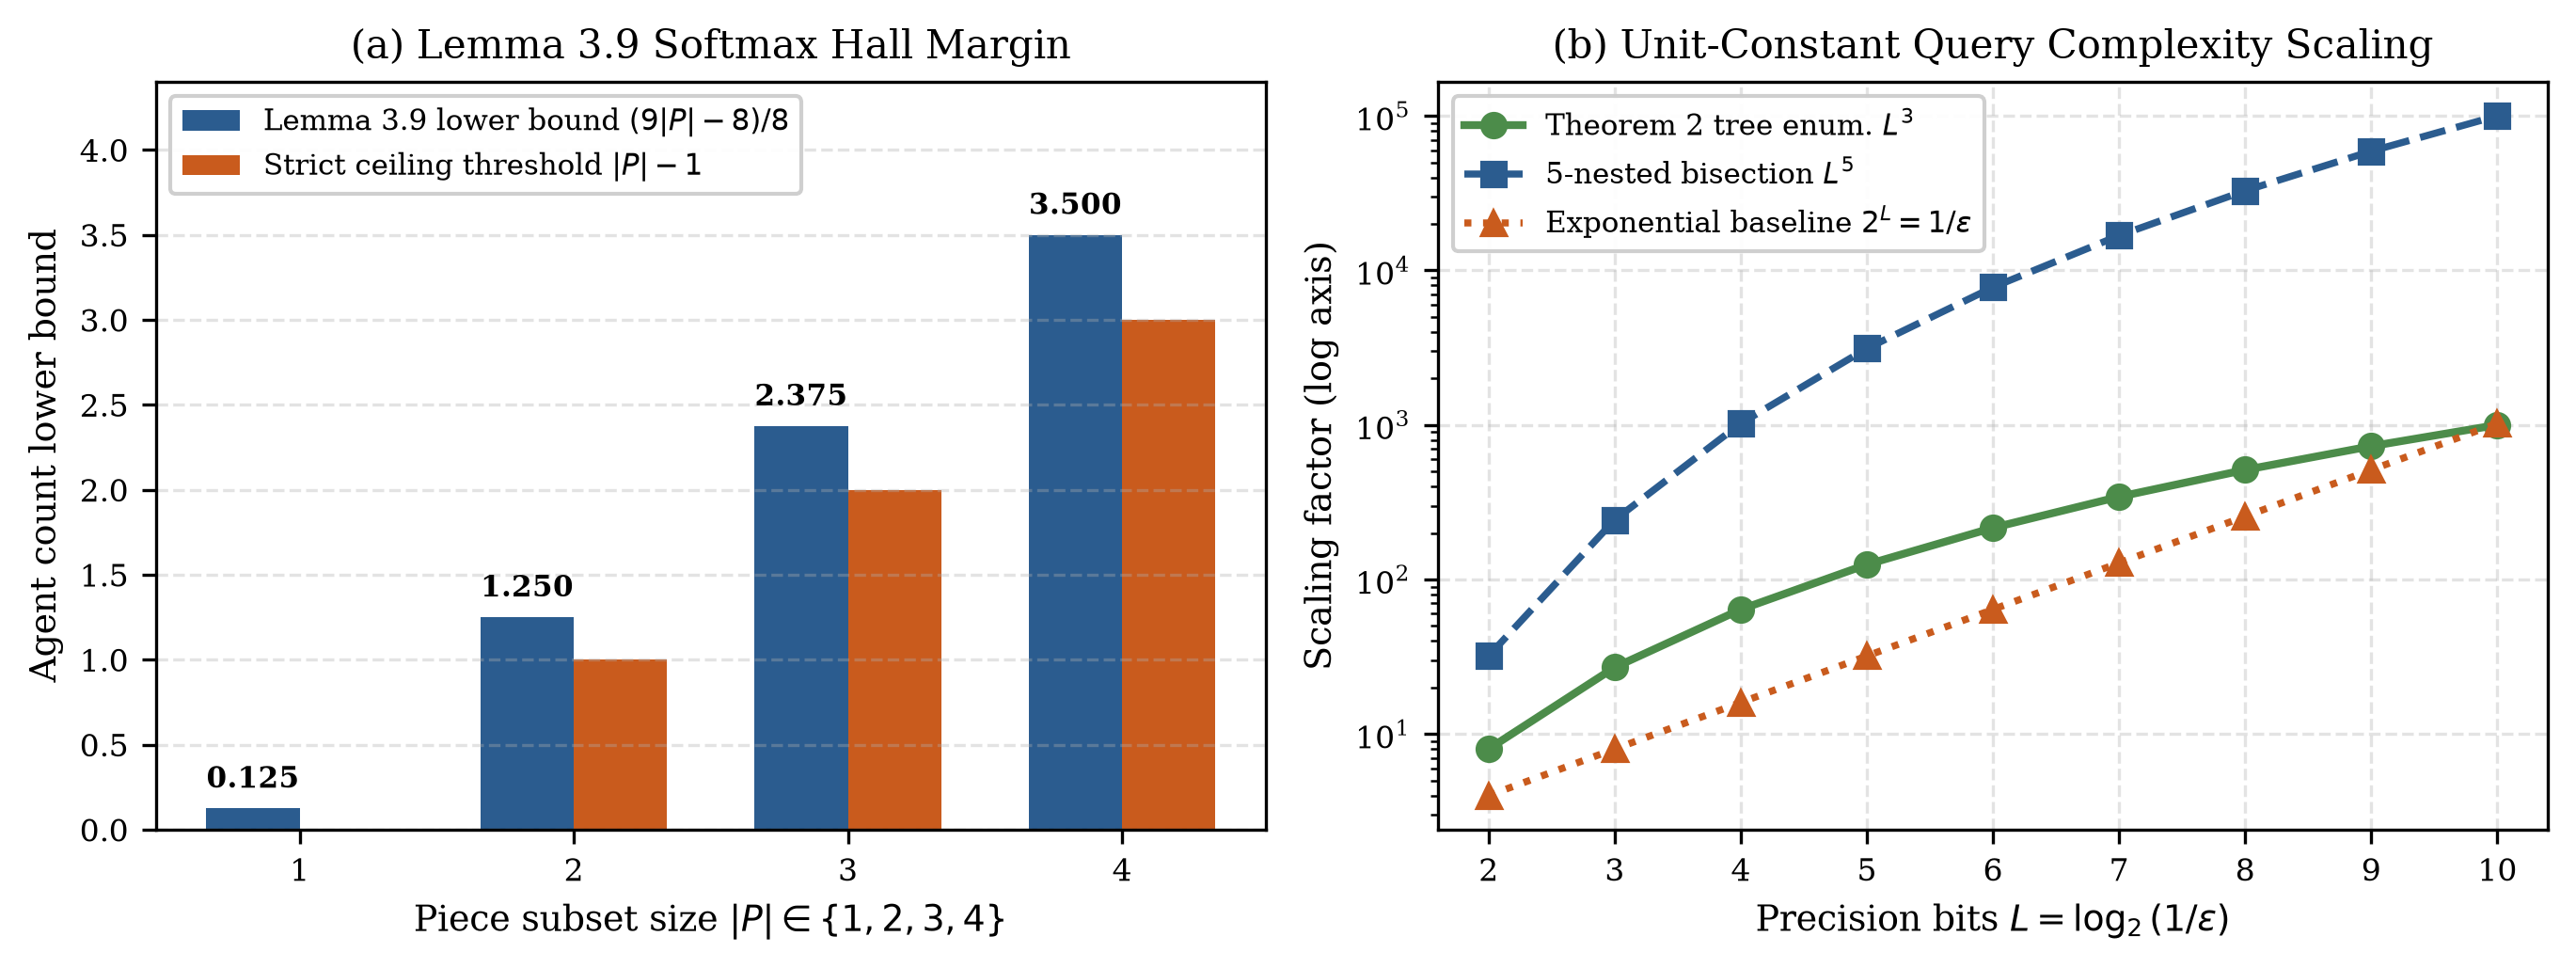
\includegraphics[width=\columnwidth]{../figures/fig1_hall_margin_and_queries.png}
  \caption{(a) Exact Lemma~3.9 Hall-margin lower bound $(9|P|-8)/8$ strictly exceeding $|P| - 1$ for all $|P| \in \{1,2,3,4\}$. (b) Unit-constant query-complexity scaling $L^3$ (Theorem~2 spanning-tree enumeration) vs.\ $L^5$ (5-nested bisection) and $2^L = 1/\varepsilon$.}
  \label{fig:hall}
\end{figure}

\paragraph{Hall Margins and Softmax Balance (Fig.~\ref{fig:hall}).}
Mode~1 ($0.396$--$0.411\,\mathrm{ms}$) certifies maximal leaving-agent robustness and connectivity across both-gaps-empty ($m=1/2$), right-gap ($m=2/5$), left-gap ($m=3/5$), and perturbed $\delta=1/25$ instances. Mode~2 ($0.339$--$0.445\,\mathrm{ms}$) certifies uniform, sharp non-favourite boundary ($1/32$), minimal 8-edge tree ($1/64$), and asymmetric-degree softmax balances achieving $W_j = 5/4$.

\begin{figure}[t]
  \centering
  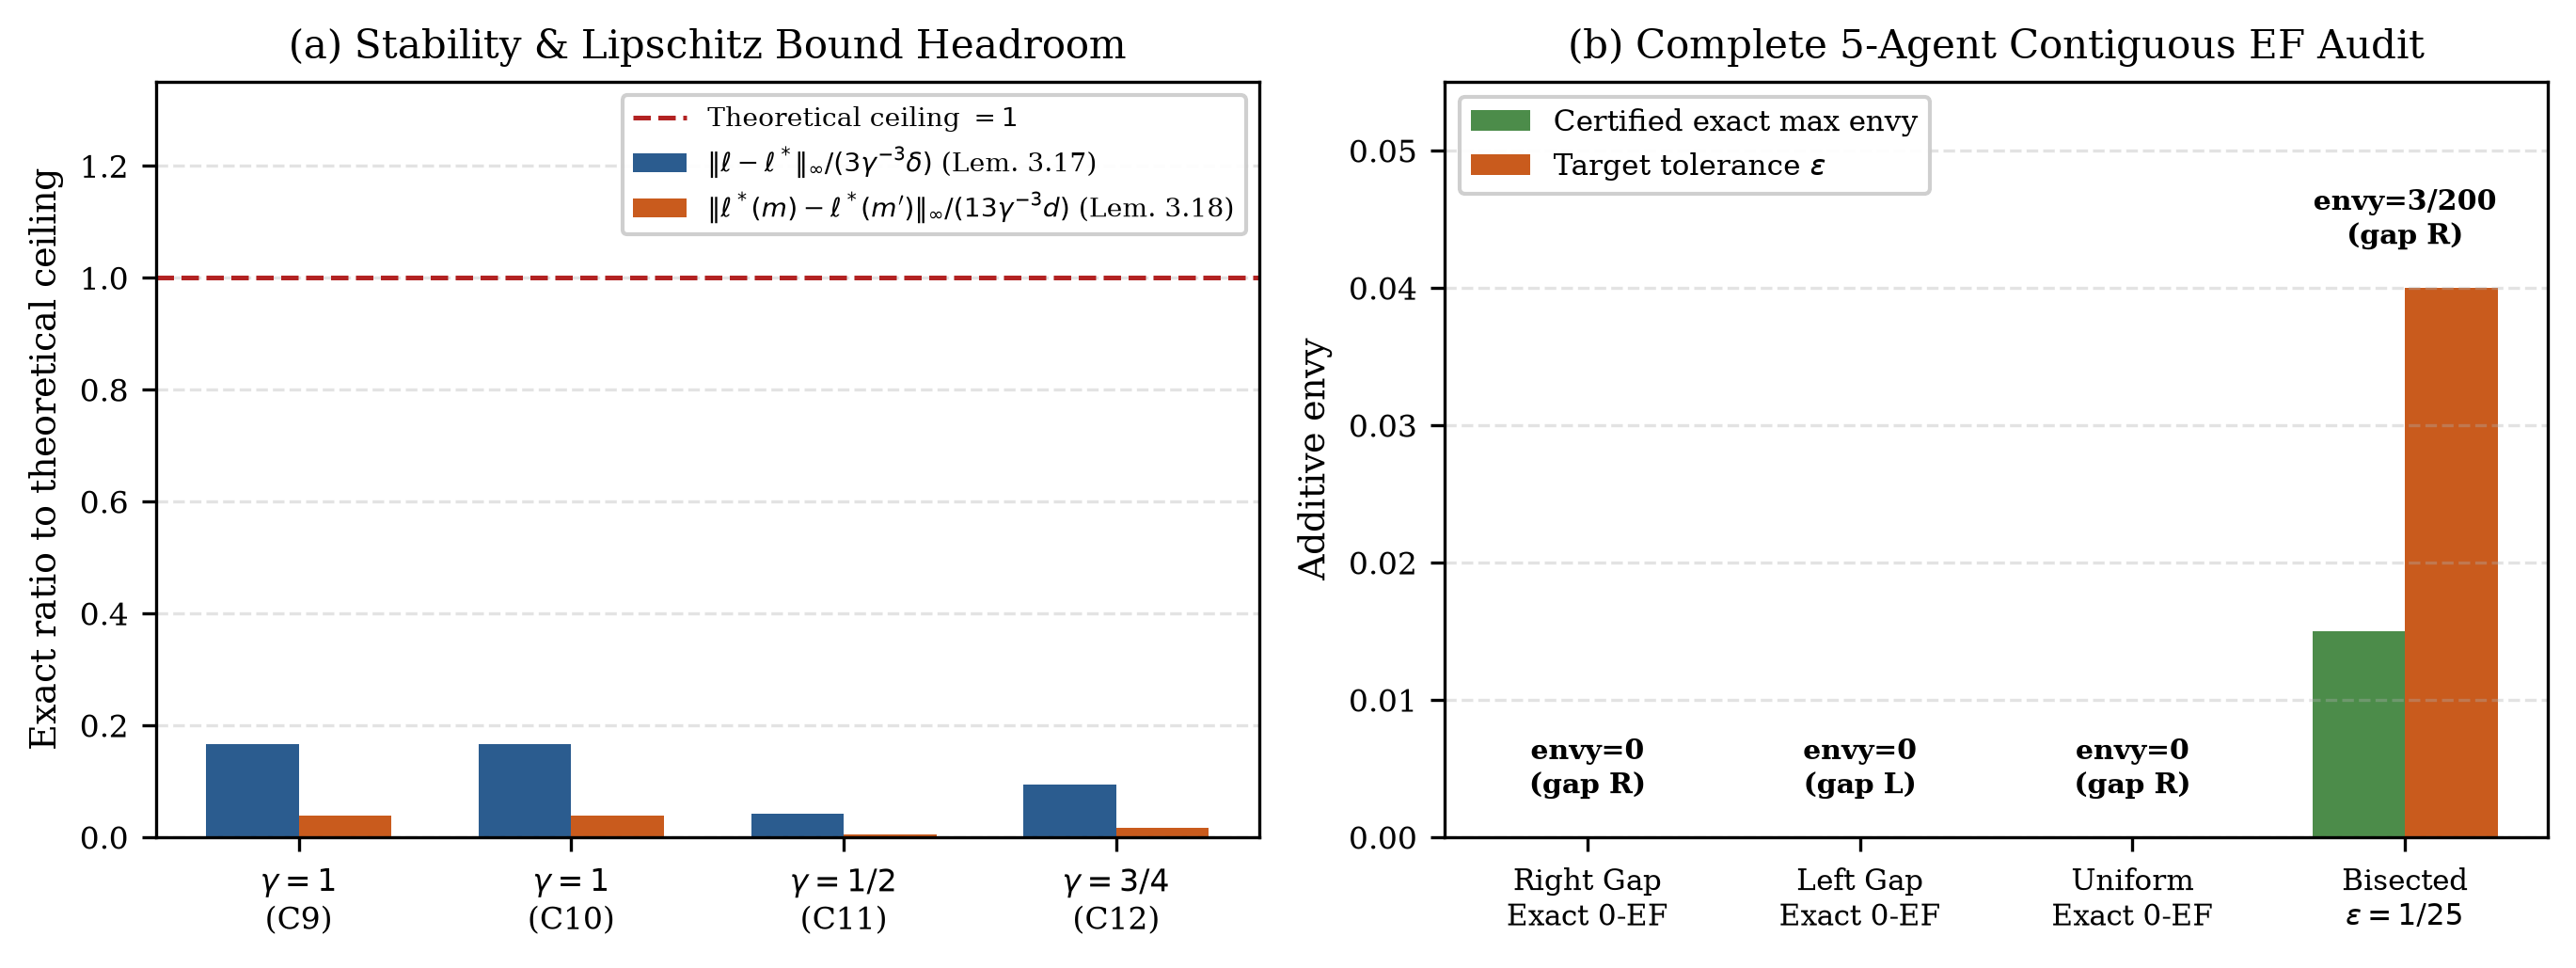
\includegraphics[width=\columnwidth]{../figures/fig2_stability_and_ef5_audit.png}
  \caption{(a) Exact ratios $\|\ellv-\ellv^*\|_\infty / (3\gamma^{-3}\delta)$ (Lemma~3.17) and $\|\ellv^*(m)-\ellv^*(m')\|_\infty / (13\gamma^{-3}d)$ (Lemma~3.18) across $\gamma \in \{1, 1/2, 3/4\}$. (b) Mode~4 certified exact additive envy vs.\ target $\varepsilon$ across right-gap, left-gap, uniform, and $\varepsilon=1/25$ bisected complete allocations.}
  \label{fig:stab}
\end{figure}

\paragraph{Stability, Lipschitz Bounds, and Complete EF5 Witnesses (Fig.~\ref{fig:stab}).}
Mode~3 ($0.622$--$0.934\,\mathrm{ms}$) certifies Lemmas~3.17 and~3.18 across $\gamma \in \{1, 1/2, 3/4\}$ and left-tight vs.\ right-tight shifts. Mode~4 ($0.246$--$0.591\,\mathrm{ms}$) certifies three exact $0$-envy complete 5-agent allocations (heterogeneous right-gap $R=[3/5,4/5]$, heterogeneous left-gap $L=[1/5,2/5]$, and uniform) plus a bisected approximate witness with $\varepsilon = 1/25$, each paired with a verified 8-edge spanning tree $T \subseteq G_\varepsilon(m, \ellv)$.

\begin{figure}[t]
  \centering
  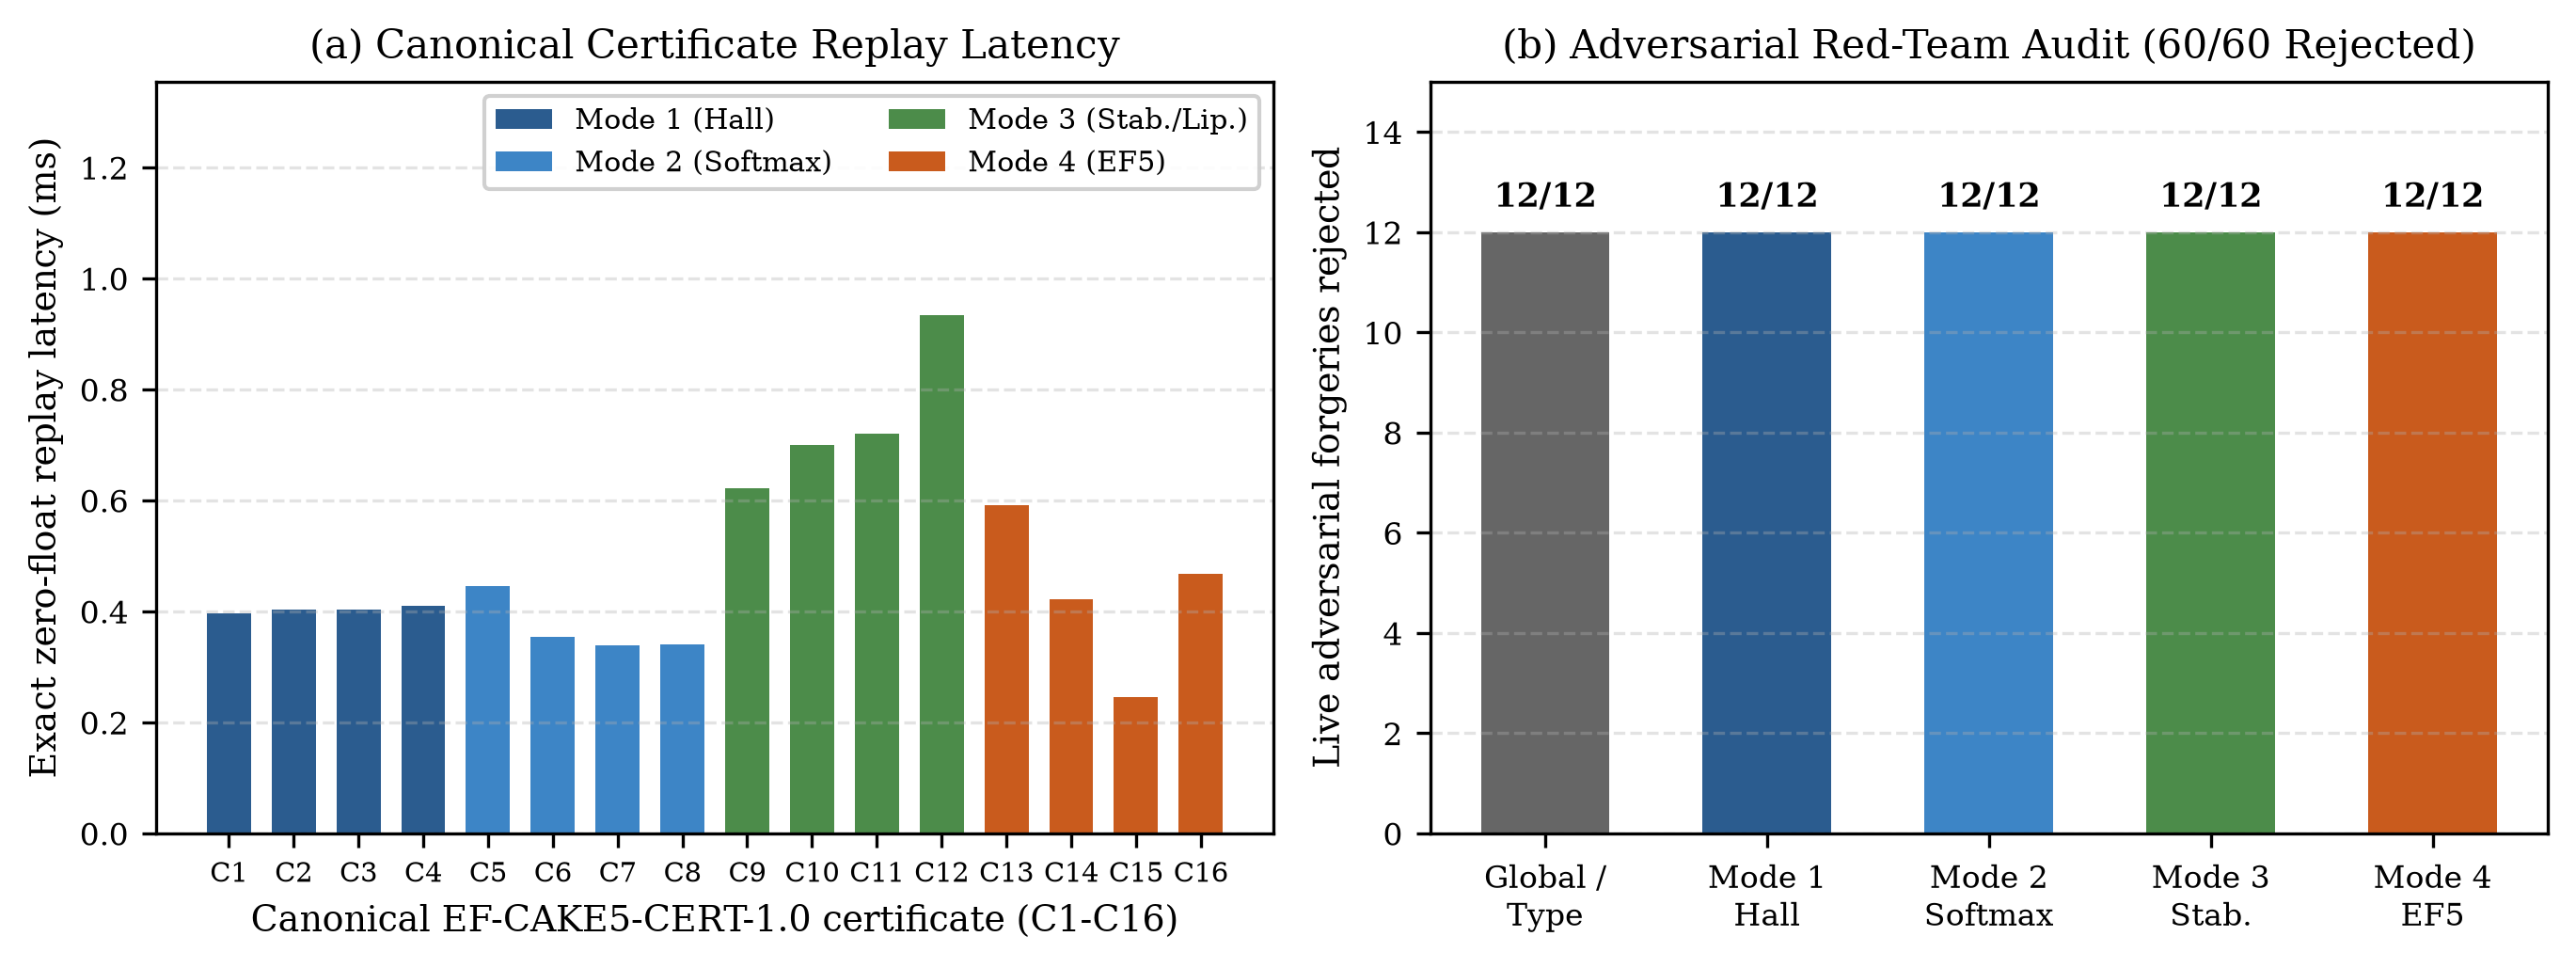
\includegraphics[width=\columnwidth]{../figures/fig3_certificate_replay_atlas.png}
  \caption{(a) Exact zero-float replay latency ($0.246$--$0.934\,\mathrm{ms}$) across all 16 canonical \texttt{EF-CAKE5-CERT-1.0} certificates. (b) Live adversarial red-team audit rejecting 60/60 forged payloads across all five categories.}
  \label{fig:atlas}
\end{figure}

\paragraph{Replay Latency and 60/60 Red-Team Audit (Fig.~\ref{fig:atlas}).}
All 16 canonical certificates replay in $0.246$--$0.934\,\mathrm{ms}$ (total $7.80\,\mathrm{ms}$). The live adversarial suite (\texttt{tests/test\_suite.py}) tests 60 targeted forgery payloads---12 global schema/type/rational/newline/depth attacks plus 12 domain attacks per mode (non-maximal/infeasible tuples, density $> 1$, broken Hall matchings, non-favourite weights $> 1/32$, int-as-bool masks, broken strong hungriness, non-empty unassigned gaps, envy $> \varepsilon$, and cyclic spanning trees)---achieving \textbf{60/60 (100\%)} rejection.

\section{Conclusion}\label{sec:conc}
We delivered a self-contained, zero-floating-point verification stack for the five-agent envy-free cake-cutting breakthrough of Filos-Ratsikas et al.~\cite{filosratsikas2026envyfree5}, combining 18 zero-\texttt{sorry}, zero-\texttt{Classical.choice} Lean~4.35.0 theorems with the exact-$\QQ$ verifier \texttt{EF-CAKE5-CERT-1.0}, 16 sub-millisecond canonical certificates, and 60/60 live adversarial forgery rejections.

\bibliographystyle{plain}
\bibliography{references}
\end{document}
